\chapter{Automatic Project Group Assignment}\label{sec:project-groups}

\cxone allows projects to be assigned to zero or more groups.  The groups are typically
used to limit visibility of scan results to users that would need to view and triage
scan results.  By default, \cxoneflow does not assign projects to groups.  An optional
configuration will allow \cxoneflow to assign projects to groups upon creation.  The
configuration can optionally update an existing project with configured group assignments
when orchestrating a scan.


\section{Assignment Logic}

Groups are assigned by defining one or more regular expressions that are applied to the clone
URL at the time a scan is orchestrated.  One or more of the regular expressions can match
the clone URL; this provides a way to select multiple groups of groups to assign to a project.
Upon project creation, the project is assigned to the matching groups.

Existing projects can optionally be updated with matching groups.  When a scan is orchestrated, the
project where the scan will execute is evaluated for group membership.  If any of the groups that
should be assigned due to the configured group membership logic are missing, the project will be
assigned to any missing groups.

Group assignments are additive in that new group assignments are added to any existing groups. If
groups are manually assigned to a project, those groups are not removed.  


\section{Configuration}

The example YAML file found with the \cxoneflow release artifacts is shown in Figure
\ref{fig:group-yaml}. The sub-elements of the \texttt{project-groups}
element configure the logic used to select zero or more groups to assign to a
\cxone project.  The grouping configuration can be used in a service definition for any
supported SCM type.

\begin{figure}[h]
    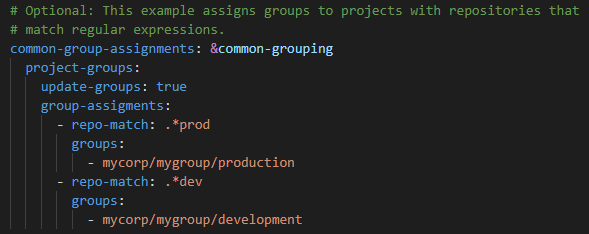
\includegraphics[width=\textwidth]{graphics/group-yaml.png}
    \caption{Group Assignment YAML Definitions}
    \label{fig:group-yaml}
\end{figure}


\subsection{The \texttt{project-groups.update-groups} YAML Element}

The \texttt{update-groups} configuration element is optional and defaults to False.  If set to True,
project group membership is evaluated at the time of scan orchestration.  If the project configuration
is found to be missing any groups that would have been assigned upon project creation, the project settings
are updated with the missing group assignments.

\subsection{The \texttt{project-groups.group-assignments} YAML Element}

The \texttt{group-assignments} element is a list of YAML dictionaries, each dictionary containing
two configuration elements.

\subsubsection{repo-match}

The \texttt{repo-match} configuration element is a regular expression applied to the clone URL.  If the
regular expression matches, the groups defined in the sibling \texttt{groups} element are assigned
to the project.  If the clone URL matches the \texttt{repo-match} of more than one entry in the
\texttt{group-assignments} list, the project is assigned to the groups in the set of all matching groups.

If the clone URL matches none of the \texttt{repo-match} entries, no groups are automatically assigned
to the project.

\subsubsection{groups}

The \texttt{groups} element is a list of group paths to which a project will be assigned when the clone URL
is matched by the regular expression in the sibling \texttt{repo-match} element.  The group should be the full
path to the group for assignment.

If an invalid group is specified in the configuration, the invalid group will be ignored.

